\section{Overall system architecture and services}
\begin{itemize}
	\item cf. \ref{fig:system-overview}
	\item \todo{highlight the differences between optimal (proposed) infrastructure and the implementation}
\end{itemize}

\begin{figure}[h]
	\centering
	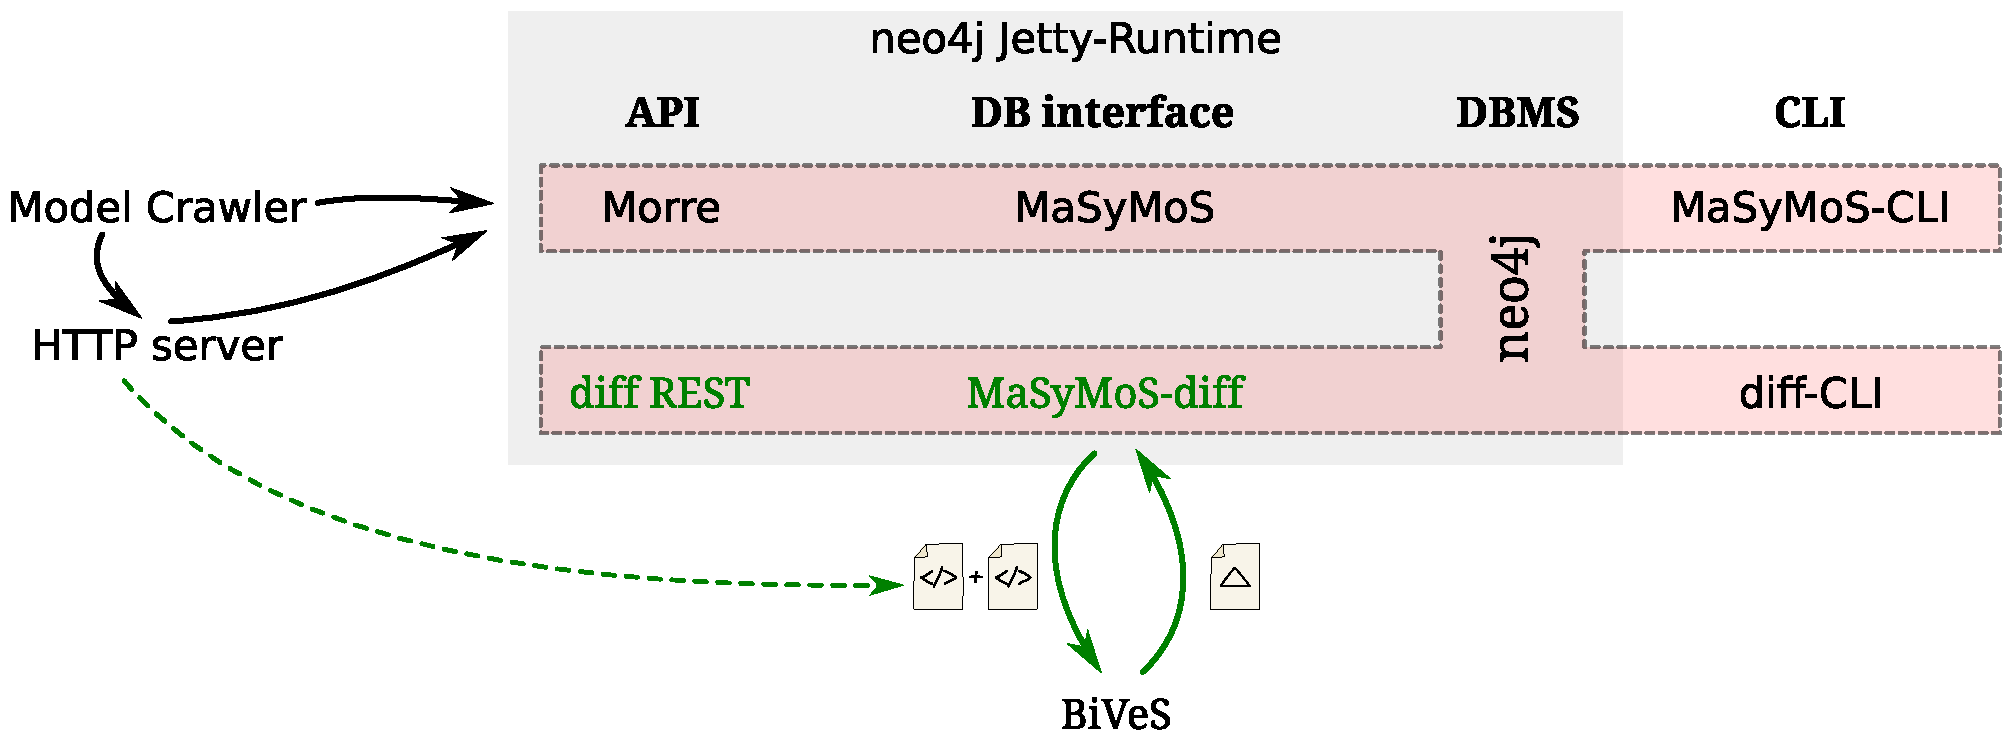
\includegraphics[width=\textwidth]{resources/system-overview-matrix.pdf}
	\caption{Infrastructure overview}
	\label{fig:system-overview}
\end{figure}

\section{Database model and storage decisions}
\begin{itemize}
\item extension to database model cf. \ref{fig:db-model}
	\subitem linking version
	\subitem storing differences
\item decisions on storage model
	\subitem storing each version full (no delta-storag)
	\subitem each version is aware to the search index
	\subitem diff still enables for analysis of changes
	\subitem higher storage consumption
\item extended storage model
\end{itemize}

\begin{figure}
	\centering
	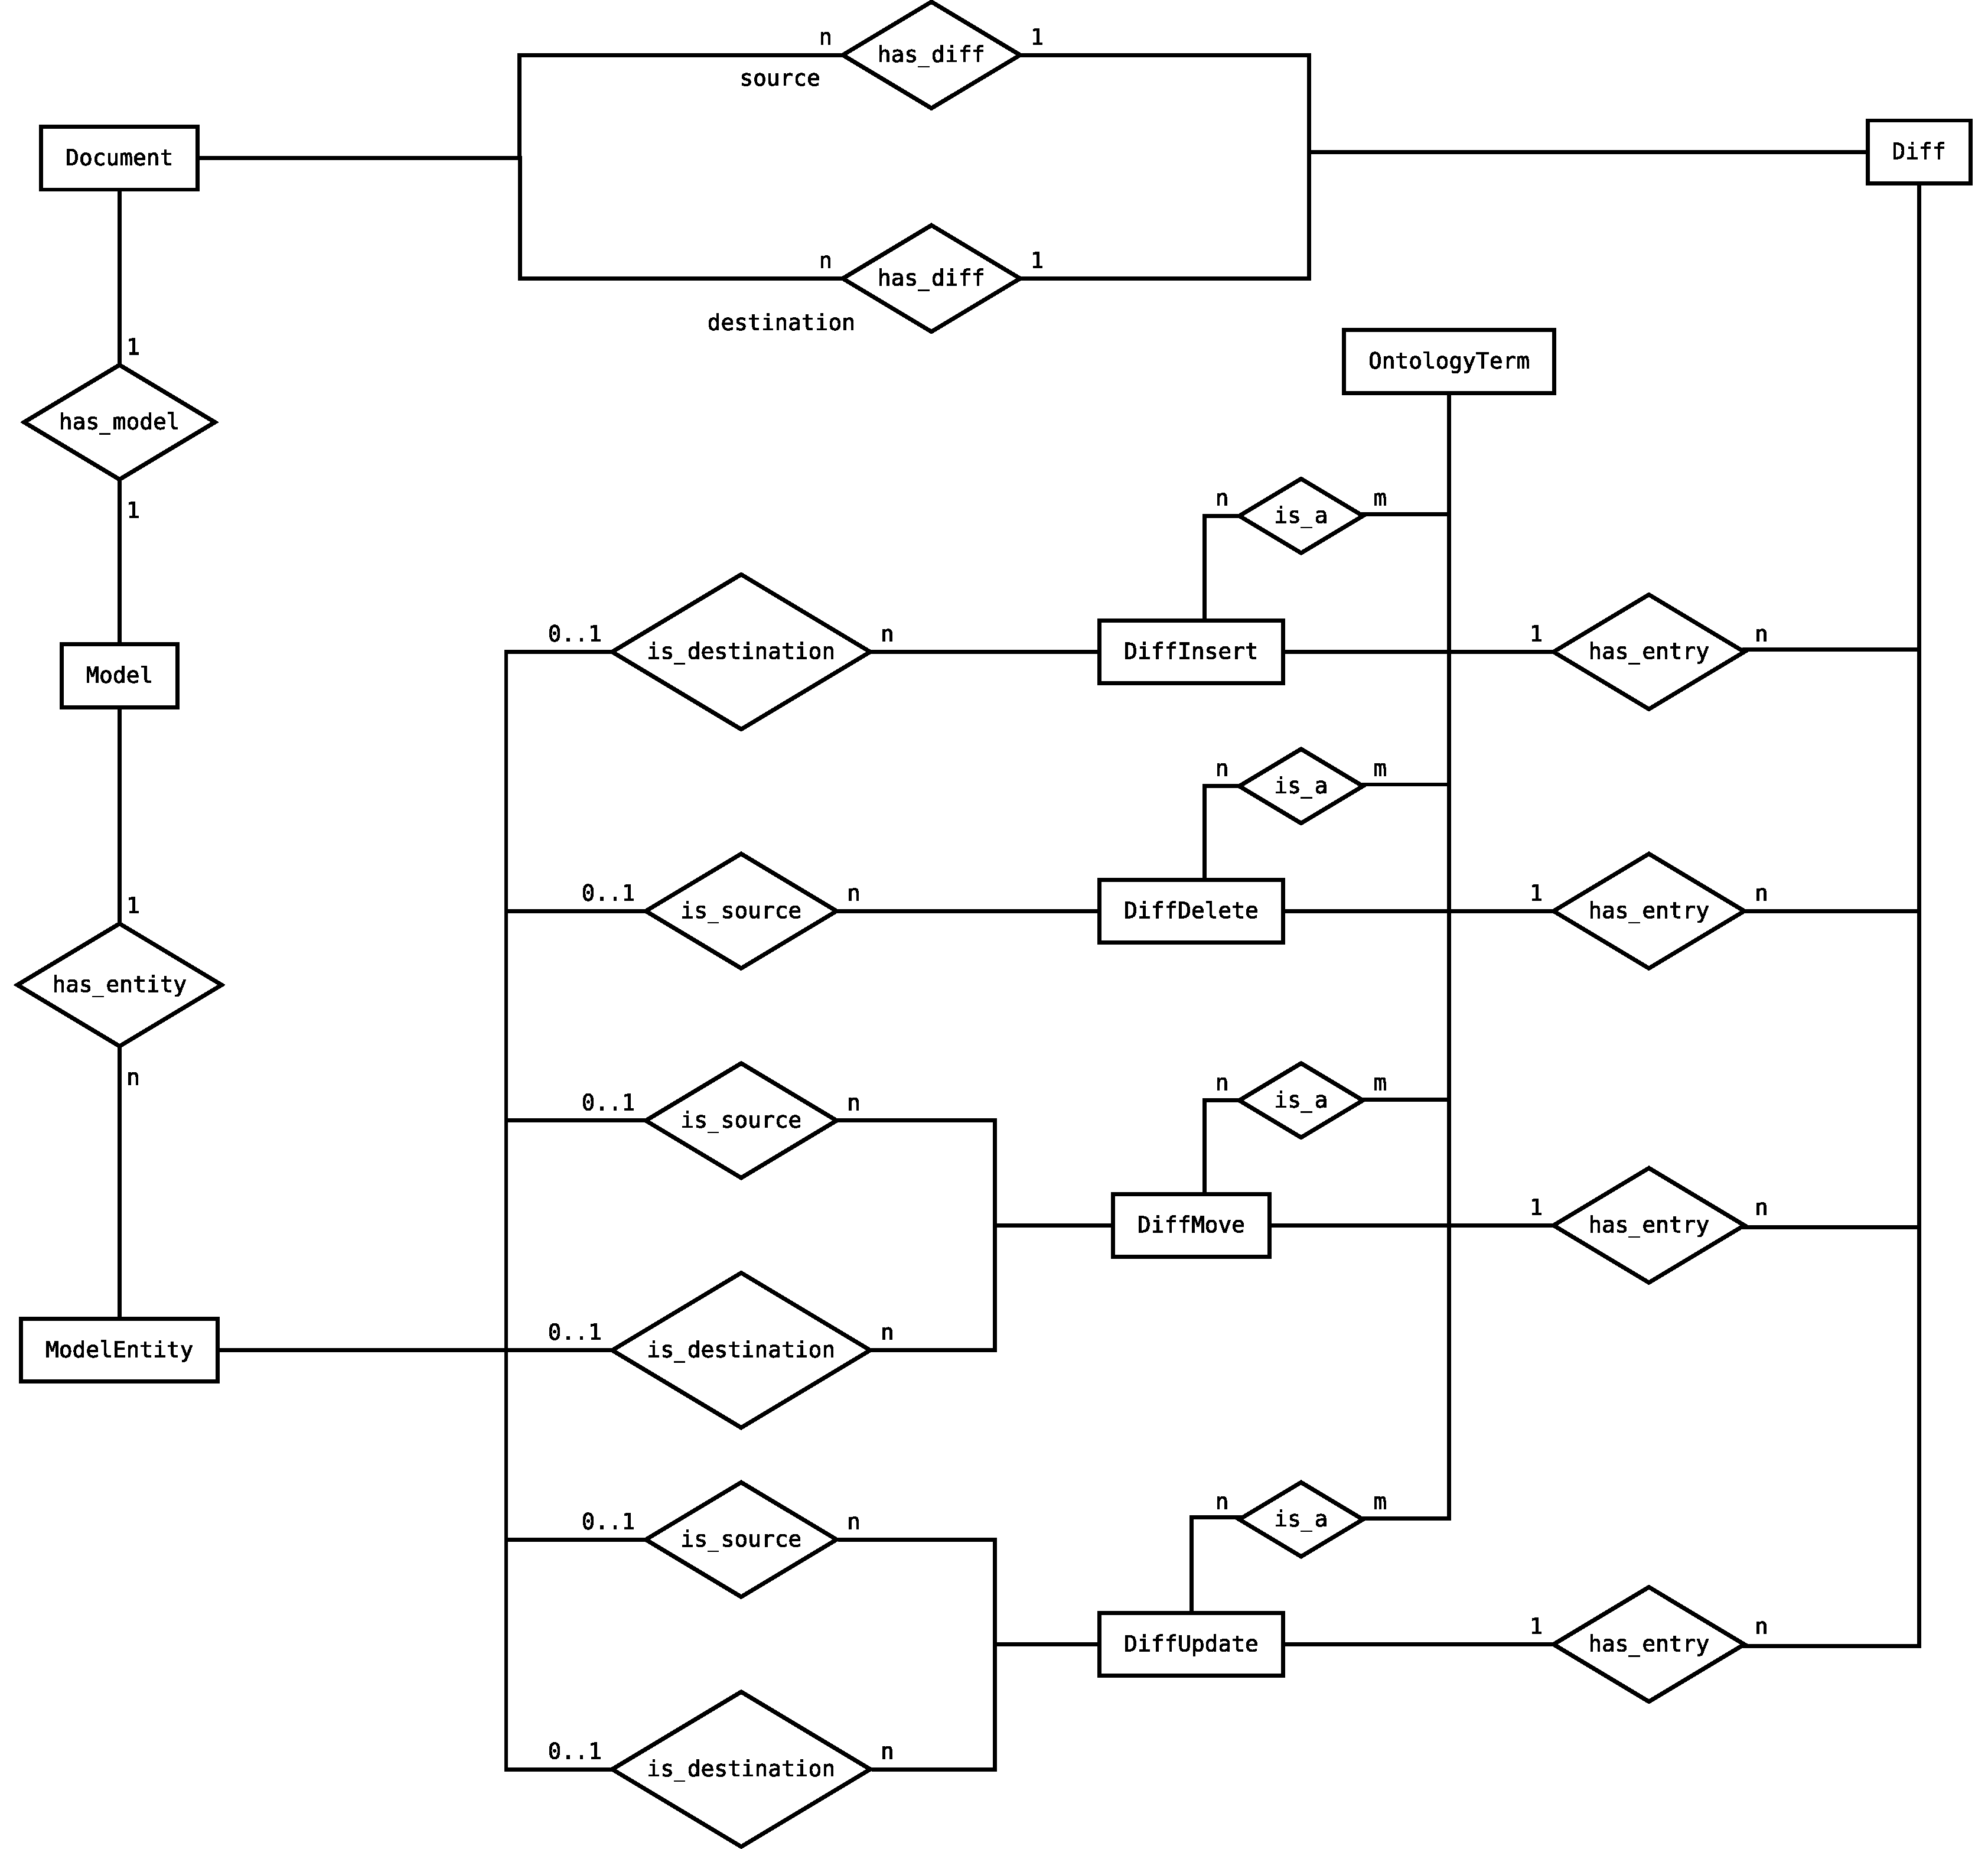
\includegraphics[width=\textwidth]{resources/db-concept-er.pdf}
	\caption{ER model of the proposed database schema}
	\label{fig:db-er-model}
\end{figure}

\begin{figure}[h]
	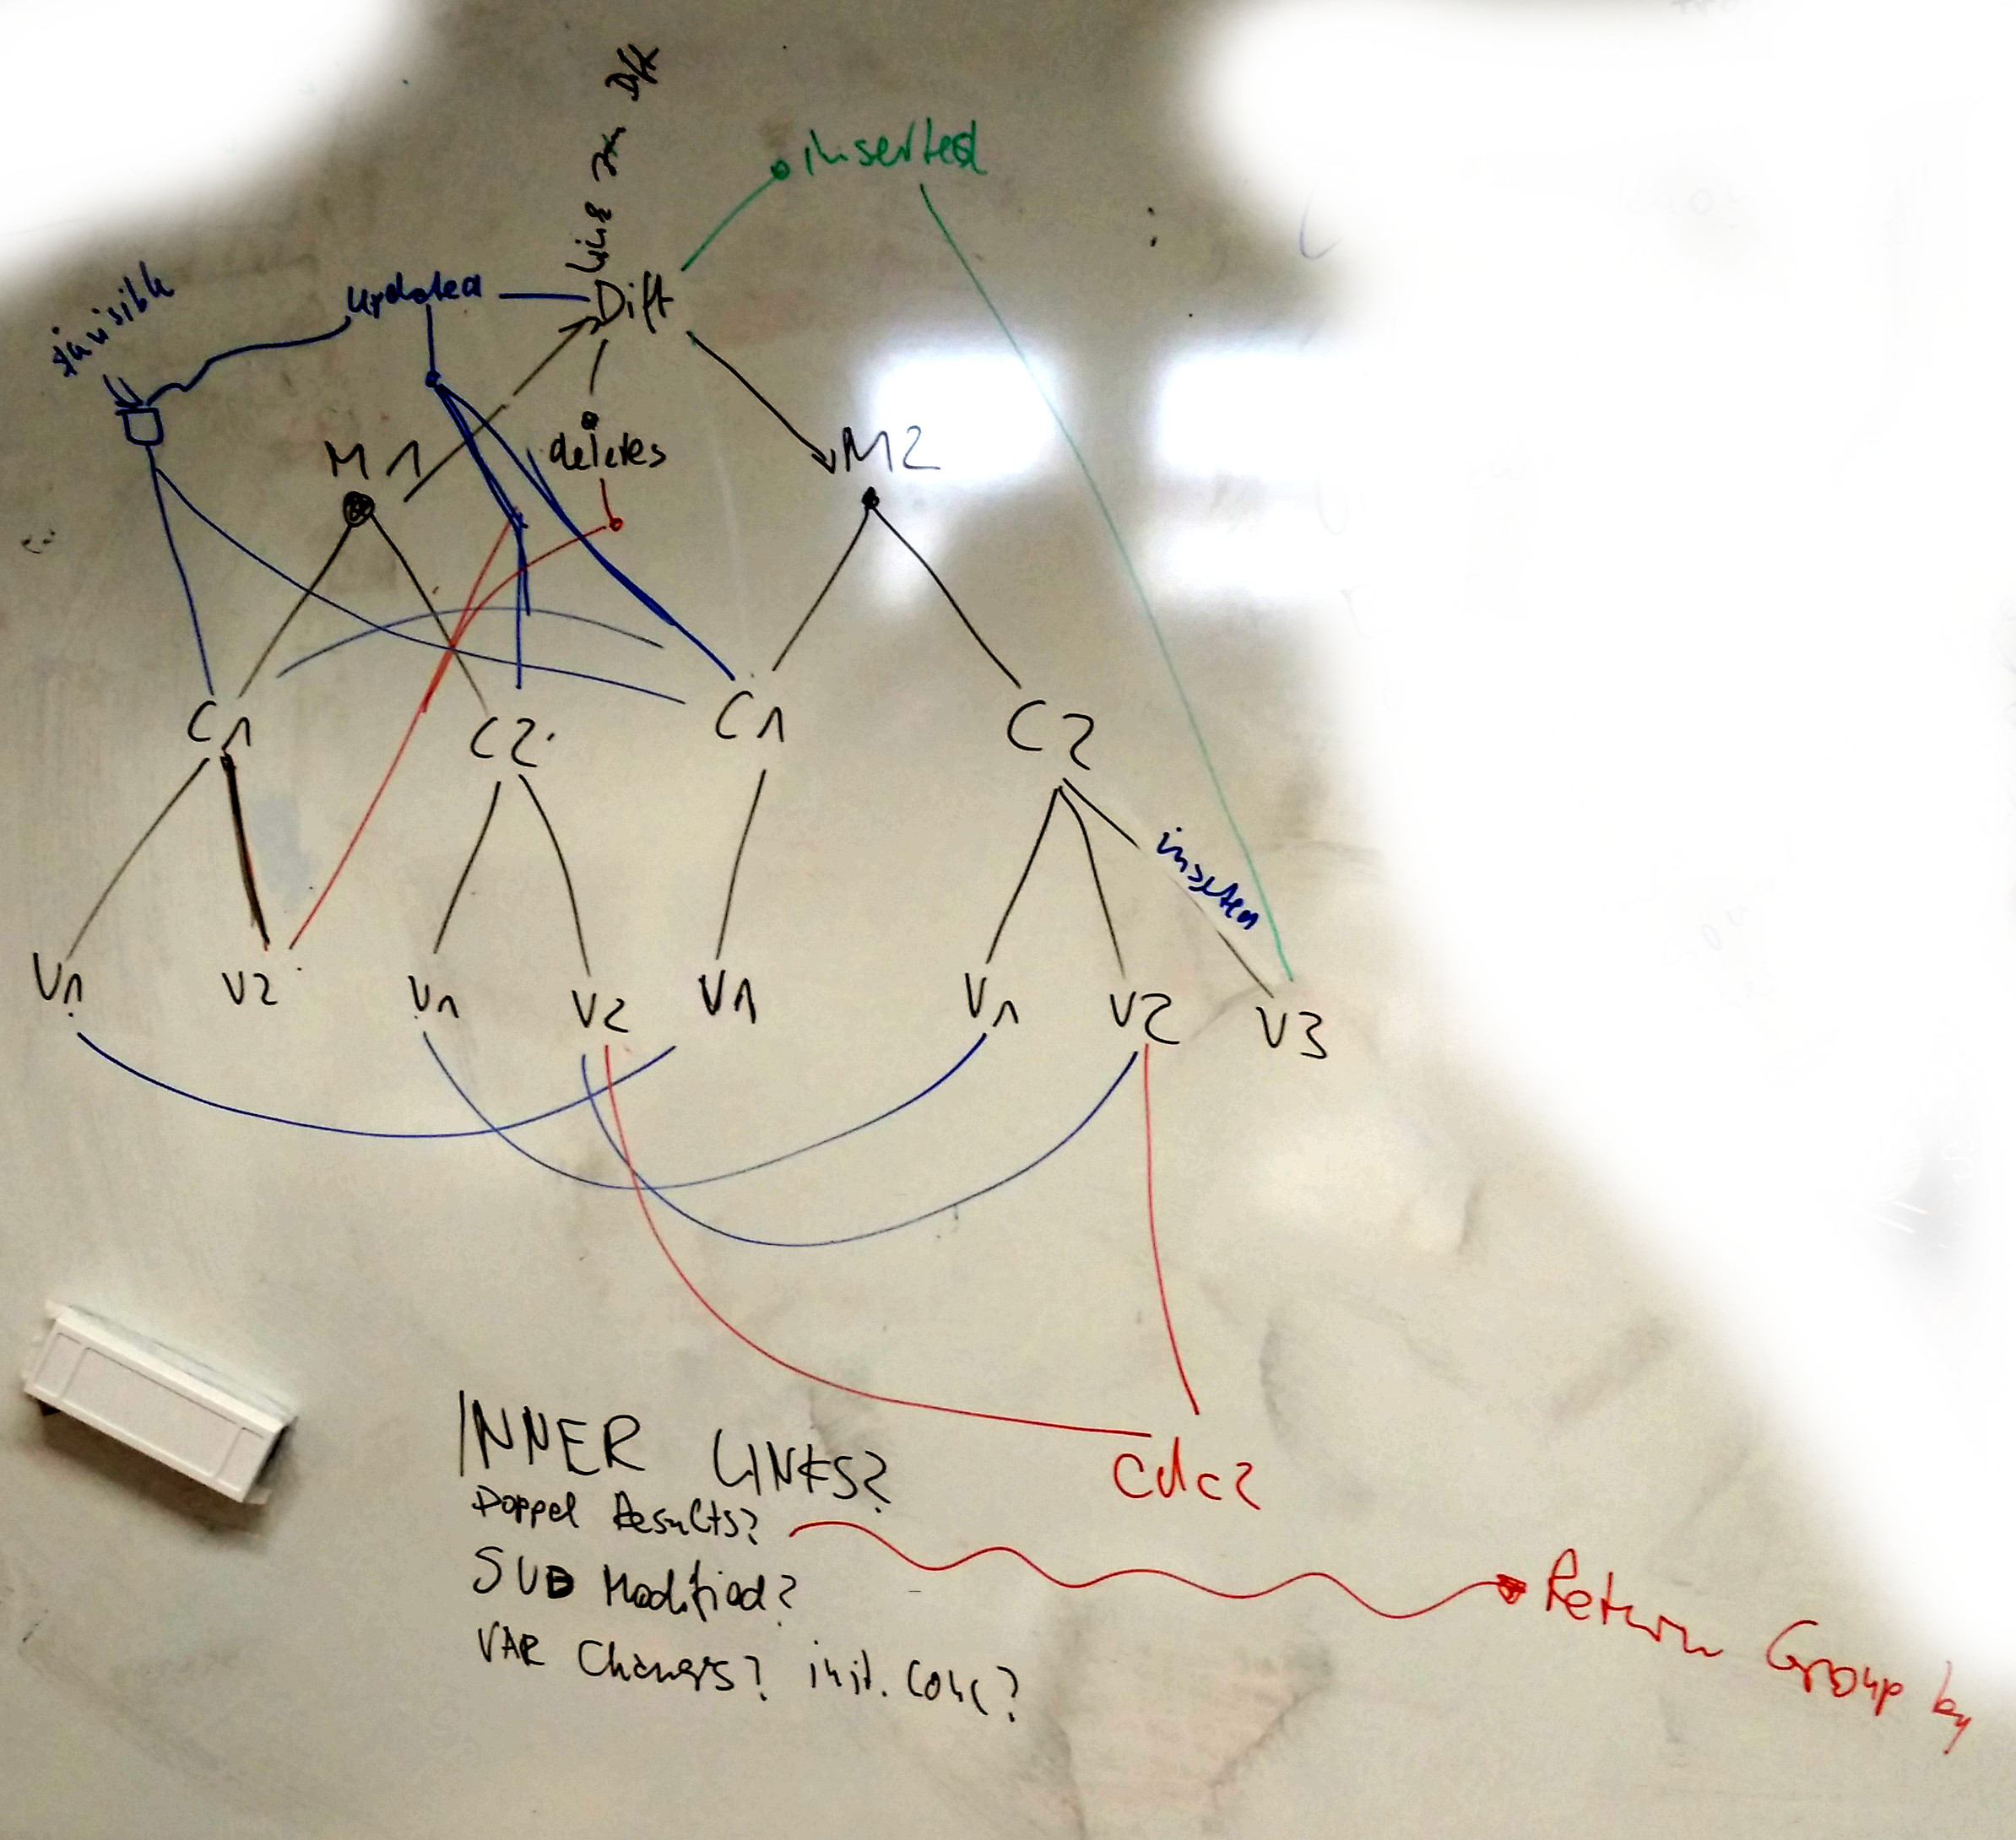
\includegraphics[width=\textwidth]{resources/db_structure.jpg}
	\caption{Proposed database structure}
	\label{fig:db-model}
\end{figure}
